\begin{enumerate}[label=\thesubsection.\arabic*, ref=\thesubsection.\theenumi]
\item
Find the domain of the function $f\brak{x} = \cos^{-1}x + \sin x$.
\hfill (CBSE Class 12, 65/7/1, Q.2)
% TODO: add options (A)-(D) from the paper; the answer is option (C)

\solution
$\cos^{-1}x$ is defined only for $-1 \le x \le 1$, and $\sin x$ is defined for every real $x$. The domain of the sum is the intersection of the two domains:
\begin{align}
	\text{Domain}\brak{f} = \sbrak{-1,1} \quad \brak{\text{Option C}}
\end{align}
The program scans $x$ over $\sbrak{-3,3}$ and treats the points where \texttt{acos(x)+sin(x)} is not a number as outside the domain. The following code verifies the solution
\begin{lstlisting}[frame=single, basicstyle=\rmfamily, escapeinside={(*@}{@*)}]
(*@\makebox[\dimexpr\linewidth-2\fboxsep-2\fboxrule\relax][c]{codes/2.c}@*)
\end{lstlisting}

\item
The number of all possible matrices of order $3 \times 3$ with each entry $2$ or $3$ is
\hfill (CBSE Class 12, 65/7/1, Q.3)
% TODO: add options (A)-(D) from the paper; the answer is option (B)

\solution
Each of the $9$ entries can independently be $2$ or $3$. By the multiplication principle,
\begin{align}
	N = 2^9 = 512 \quad \brak{\text{Option B}}
\end{align}
The following code verifies the solution
\begin{lstlisting}[frame=single, basicstyle=\rmfamily, escapeinside={(*@}{@*)}]
(*@\makebox[\dimexpr\linewidth-2\fboxsep-2\fboxrule\relax][c]{codes/3.c}@*)
\end{lstlisting}

\item
The matrix $\vec{A} = \myvec{3 & 0 & 0 \\ 0 & 2 & 0 \\ 0 & 0 & 5}$ is a
\hfill (CBSE Class 12, 65/7/1, Q.4)
\begin{enumerate}
	\begin{multicols}{4}
    \item scalar matrix
    \item identity matrix
    \item null matrix
    \item symmetric matrix
	\end{multicols}
\end{enumerate}

\solution
(theory only) A matrix is symmetric if $\vec{A}^{\top} = \vec{A}$. For a diagonal matrix the transpose leaves every entry unchanged,
\begin{align}
	\vec{A}^{\top} = \myvec{3 & 0 & 0 \\ 0 & 2 & 0 \\ 0 & 0 & 5} = \vec{A}
\end{align}
The diagonal entries are not all equal, so $\vec{A}$ is not a scalar matrix; it is neither the identity nor the null matrix. Hence $\vec{A}$ is a symmetric matrix $\brak{\text{Option D}}$.

\item
If $\vec{A}$ and $\vec{B}$ are square matrices of order $3$ with $\abs{\vec{A}} = 3$ and $\abs{\vec{B}} = 5$, then $\abs{2\vec{A}\vec{B}}$ is
\hfill (CBSE Class 12, 65/7/1, Q.5)
% TODO: add options (A)-(D) from the paper; the answer is option (B)

\solution
For an $n \times n$ matrix, $\abs{k\vec{A}} = k^n\abs{\vec{A}}$ and $\abs{\vec{A}\vec{B}} = \abs{\vec{A}}\abs{\vec{B}}$. With $n = 3$,
\begin{align}
	\abs{2\vec{A}\vec{B}} = 2^3\abs{\vec{A}}\abs{\vec{B}} = 8\brak{3}\brak{5} = 120 \quad \brak{\text{Option B}}
\end{align}
Standard C has no built-in determinant routine, so the program defines \texttt{det3()} using cofactor expansion and applies it to the product matrix $2\vec{A}\vec{B}$. The following code verifies the solution
\begin{lstlisting}[frame=single, basicstyle=\rmfamily, escapeinside={(*@}{@*)}]
(*@\makebox[\dimexpr\linewidth-2\fboxsep-2\fboxrule\relax][c]{codes/5.c}@*)
\end{lstlisting}

\item
If $\vec{A}$ is a square matrix of order $3$ with $\abs{\vec{A}} = 5$, then $\abs{\text{adj}\,\vec{A}}$ is
\hfill (CBSE Class 12, 65/7/1, Q.6)
% TODO: add options (A)-(D) from the paper; the answer is option (C)

\solution
For an $n\times n$ matrix, $\vec{A}\,\text{adj}\,\vec{A} = \abs{\vec{A}}\vec{I}$. Taking determinants,
\begin{align}
	\abs{\vec{A}}\abs{\text{adj}\,\vec{A}} = \abs{\vec{A}}^n \implies \abs{\text{adj}\,\vec{A}} = \abs{\vec{A}}^{n-1}
\end{align}
For $n = 3$,
\begin{align}
	\abs{\text{adj}\,\vec{A}} = 5^2 = 25 \quad \brak{\text{Option C}}
\end{align}
The program builds $\text{adj}\,\vec{A}$ from cofactors and applies the same \texttt{det3()} function. The following code verifies the solution
\begin{lstlisting}[frame=single, basicstyle=\rmfamily, escapeinside={(*@}{@*)}]
(*@\makebox[\dimexpr\linewidth-2\fboxsep-2\fboxrule\relax][c]{codes/6.c}@*)
\end{lstlisting}

\item
The function $f\brak{x} = 2x - \sin x$, $x \in \mathbb{R}$, is
\hfill (CBSE Class 12, 65/7/1, Q.11)
% TODO: add options (A)-(D) from the paper; the answer is option (B)

\solution
Differentiating,
\begin{align}
	f^{\prime}\brak{x} = 2 - \cos x
\end{align}
Since $-1 \le \cos x \le 1$,
\begin{align}
	1 \le f^{\prime}\brak{x} \le 3 \implies f^{\prime}\brak{x} > 0 \quad \forall x \in \mathbb{R}
\end{align}
A differentiable function with a strictly positive derivative is strictly increasing, so $f$ is strictly increasing on $\mathbb{R}$ $\brak{\text{Option B}}$. The program classifies each scanned point with \texttt{if-else} on the sign of $f^{\prime}\brak{x}$. The following code verifies the solution
\begin{lstlisting}[frame=single, basicstyle=\rmfamily, escapeinside={(*@}{@*)}]
(*@\makebox[\dimexpr\linewidth-2\fboxsep-2\fboxrule\relax][c]{codes/11.c}@*)
\end{lstlisting}
The following code generates \figref{fig:CBSE12-q11}.
\begin{lstlisting}[frame=single, basicstyle=\rmfamily, escapeinside={(*@}{@*)}]
(*@\makebox[\dimexpr\linewidth-2\fboxsep-2\fboxrule\relax][c]{codes/11plot.py}@*)
\end{lstlisting}
\begin{figure}[H]
	\centering
	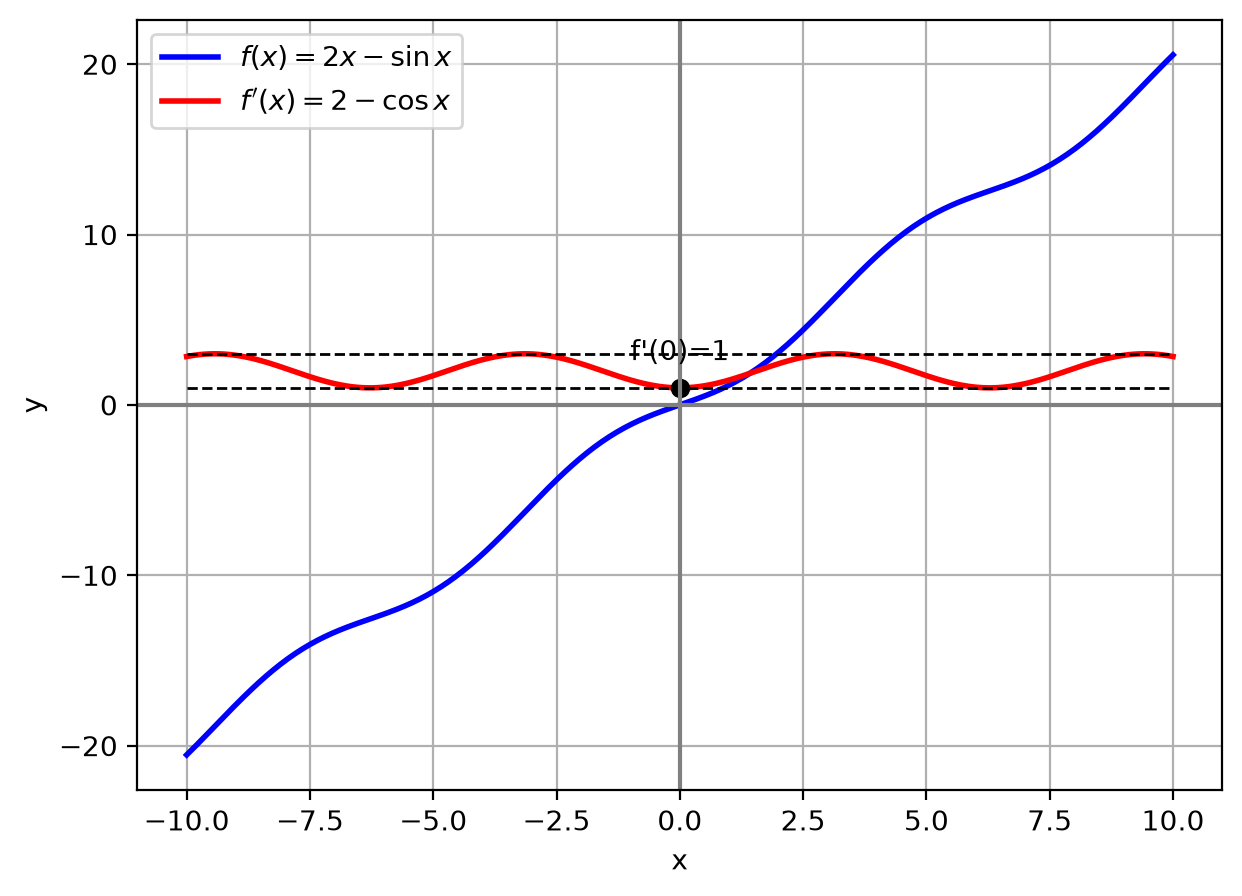
\includegraphics[width=0.7\linewidth]{figs/c12_q11.png}
	\caption{$f\brak{x}$ and $f^{\prime}\brak{x}$ with $1 \le f^{\prime}\brak{x} \le 3$}
	\label{fig:CBSE12-q11}
\end{figure}

\item
Evaluate $\displaystyle\int \frac{e^{9\log x} - e^{8\log x}}{e^{6\log x} - e^{5\log x}}\,dx$.
\hfill (CBSE Class 12, 65/7/1, Q.12)
% TODO: add options (A)-(D) from the paper; the answer is option (C)

\solution
For $x > 0$, $e^{k\log x} = x^k$. Hence, for $x \neq 1$,
\begin{align}
	\frac{x^9 - x^8}{x^6 - x^5} = \frac{x^8\brak{x-1}}{x^5\brak{x-1}} = x^3
\end{align}
\begin{align}
	\int x^3\,dx = \frac{x^4}{4} + C \quad \brak{\text{Option C}}
\end{align}
The midpoint Riemann sum $\sum_{i=1}^{n} f\brak{x_i^*}\Delta x$ of the original integrand over $\sbrak{2,4}$ is compared with $\frac{x^4}{4}\Big|_2^4 = 60$. The following code verifies the solution
\begin{lstlisting}[frame=single, basicstyle=\rmfamily, escapeinside={(*@}{@*)}]
(*@\makebox[\dimexpr\linewidth-2\fboxsep-2\fboxrule\relax][c]{codes/12.py}@*)
\end{lstlisting}

\item
Which of the following statements is correct?
\hfill (CBSE Class 12, 65/7/1, Q.13)
\begin{enumerate}[label=(\Alph*)]
	\item $\displaystyle\int_a^b f\brak{x}\,dx = \int_a^b f\brak{a+b-x}\,dx$
	\item $\displaystyle\int_{-a}^{a} f\brak{x}\,dx = 0$ if $f$ is even
	\item $\displaystyle\int_{-a}^{a} f\brak{x}\,dx = 2\int_0^a f\brak{x}\,dx$ if $f$ is odd
	\item $\displaystyle\int_0^{2a} f\brak{x}\,dx = \int_0^a f\brak{x}\,dx - \int_0^a f\brak{2a+x}\,dx$
\end{enumerate}
% TODO: confirm the exact wording of options (B)-(D) against the paper

\solution
\textbf{(A)} Put $u = a+b-x$, $du = -dx$. When $x = a$, $u = b$ and when $x = b$, $u = a$, so
\begin{align}
	\int_a^b f\brak{a+b-x}\,dx = \int_b^a f\brak{u}\brak{-du} = \int_a^b f\brak{u}\,du
\end{align}
(A) is true.

\textbf{(B)} For an even function $\int_{-a}^{a} f = 2\int_0^a f$. With $f\brak{x} = x^2$, $\int_{-1}^{1}x^2\,dx = \frac{2}{3} \neq 0$. False.

\textbf{(C)} For an odd function $\int_{-a}^{a} f = 0$. With $f\brak{x} = x$, the left side is $0$ and the right side is $1$. False.

\textbf{(D)} The correct splitting is $\int_0^{2a} f = \int_0^a f + \int_0^a f\brak{a+x}\,dx$. With $f\brak{x}=x$, $a=1$, the left side is $2$ and the right side is $-2$. False.

Hence the correct statement is (A). The program checks each option with SymPy. The following code verifies the solution
\begin{lstlisting}[frame=single, basicstyle=\rmfamily, escapeinside={(*@}{@*)}]
(*@\makebox[\dimexpr\linewidth-2\fboxsep-2\fboxrule\relax][c]{codes/13.py}@*)
\end{lstlisting}

\item
Evaluate $\displaystyle\int \frac{e^x}{\sqrt{4 - e^{2x}}}\,dx$.
\hfill (CBSE Class 12, 65/7/1, Q.14)
% TODO: add options (A)-(D) from the paper; the answer is option (D)

\solution
Let $u = \frac{e^x}{2}$, so $du = \frac{e^x}{2}\,dx$ and $4 - e^{2x} = 4\brak{1 - u^2}$. Then
\begin{align}
	\int \frac{e^x\,dx}{\sqrt{4-e^{2x}}} = \int \frac{2\,du}{2\sqrt{1-u^2}} = \sin^{-1}u + C = \sin^{-1}\brak{\frac{e^x}{2}} + C \quad \brak{\text{Option D}}
\end{align}
valid for $e^{2x} < 4$, i.e.\ $x < \ln 2$. The program compares a midpoint Riemann sum over $\sbrak{-1, 0.5}$ with $F\brak{b} - F\brak{a}$. The following code verifies the solution
\begin{lstlisting}[frame=single, basicstyle=\rmfamily, escapeinside={(*@}{@*)}]
(*@\makebox[\dimexpr\linewidth-2\fboxsep-2\fboxrule\relax][c]{codes/14.py}@*)
\end{lstlisting}

\item
If $\vec{a}$ and $\vec{b}$ are two vectors such that $\abs{\vec{a}+\vec{b}} = \abs{\vec{a}-\vec{b}}$, then $\vec{a}$ and $\vec{b}$ are
\hfill (CBSE Class 12, 65/7/1, Q.16)
% TODO: add options (A)-(D) from the paper; the answer is option (A)

\solution
(theory only) Squaring both sides and using $\abs{\vec{x}}^2 = \vec{x}^{\top}\vec{x}$,
\begin{align}
	\abs{\vec{a}}^2 + 2\vec{a}^{\top}\vec{b} + \abs{\vec{b}}^2 &= \abs{\vec{a}}^2 - 2\vec{a}^{\top}\vec{b} + \abs{\vec{b}}^2
	\\
	\implies 4\vec{a}^{\top}\vec{b} &= 0
\end{align}
Hence $\vec{a}$ and $\vec{b}$ are orthogonal $\brak{\text{Option A}}$; the zero vector is the trivial case.

\item
If $\pr{A} = \frac{1}{7}$, $\pr{B} = \frac{5}{7}$ and $\pr{A \cap B} = \frac{4}{7}$, find $\pr{A^{\prime} \mid B}$.
\hfill (CBSE Class 12, 65/7/1, Q.17)
% TODO: these values are as transcribed in the chat; P(A and B) > P(A), so please
% re-check the probabilities against the paper before submitting.

\solution
By the definition of conditional probability,
\begin{align}
	\pr{A^{\prime}\mid B} = \frac{\pr{A^{\prime}\cap B}}{\pr{B}} = \frac{\pr{B} - \pr{A\cap B}}{\pr{B}}
\end{align}
This needs only $\pr{B}$ and $\pr{A\cap B}$:
\begin{align}
	\pr{A^{\prime}\mid B} = \frac{\frac{5}{7} - \frac{4}{7}}{\frac{5}{7}} = \frac{1}{5}
\end{align}
The values as printed are not consistent with each other, because an intersection cannot be more probable than $A$ alone ($\frac{4}{7} > \frac{1}{7}$); the program prints a warning for this and then evaluates the formula above. The following code verifies the solution
\begin{lstlisting}[frame=single, basicstyle=\rmfamily, escapeinside={(*@}{@*)}]
(*@\makebox[\dimexpr\linewidth-2\fboxsep-2\fboxrule\relax][c]{codes/17.c}@*)
\end{lstlisting}

\item
A coin is tossed and a card is selected at random from a well-shuffled pack of $52$ cards. The probability of getting a head and a face card is
\hfill (CBSE Class 12, 65/7/1, Q.18)
% TODO: add options (A)-(D) from the paper; the answer is option (B)

\solution
Define the indicator maps
\begin{align}
	X = \begin{cases} 1 & \text{head} \\ 0 & \text{tail} \end{cases}, \qquad
	Y = \begin{cases} 1 & \text{face card} \\ 0 & \text{otherwise} \end{cases}
\end{align}
There are $12$ face cards, so $\pr{X=1} = \frac{1}{2}$ and $\pr{Y=1} = \frac{12}{52} = \frac{3}{13}$. The two trials are independent, so the joint pmf is the product,
\begin{align}
	\pr{X=1, Y=1} = \frac{1}{2}\cdot\frac{3}{13} = \frac{3}{26} \quad \brak{\text{Option B}}
\end{align}
The following code verifies the solution
\begin{lstlisting}[frame=single, basicstyle=\rmfamily, escapeinside={(*@}{@*)}]
(*@\makebox[\dimexpr\linewidth-2\fboxsep-2\fboxrule\relax][c]{codes/18.c}@*)
\end{lstlisting}

\item
If $\vec{A} = \myvec{2 & 3 \\ -1 & 2}$, show that $\vec{A}^2 - 4\vec{A} + 7\vec{I} = \vec{0}$.
\hfill (CBSE Class 12, 65/7/1, Q.22)

\solution
The trace and determinant are
\begin{align}
	\text{tr}\brak{\vec{A}} = 2 + 2 = 4, \qquad \abs{\vec{A}} = 2\brak{2} - 3\brak{-1} = 7
\end{align}
The characteristic polynomial of a $2\times2$ matrix is $\lambda^2 - \text{tr}\brak{\vec{A}}\lambda + \abs{\vec{A}}$, so
\begin{align}
	\lambda^2 - 4\lambda + 7 = 0 \implies \lambda = \frac{4 \pm \sqrt{16-28}}{2} = 2 \pm i\sqrt{3}
\end{align}
The eigenvalues sum to $4$ (the trace) and multiply to $7$ (the determinant). By the Cayley--Hamilton theorem, $\vec{A}$ satisfies its own characteristic equation:
\begin{align}
	\vec{A}^2 - 4\vec{A} + 7\vec{I} = \vec{0}
\end{align}
Direct verification: $\vec{A}^2 = \myvec{1 & 12 \\ -4 & 1}$, $4\vec{A} = \myvec{8 & 12 \\ -4 & 8}$, $7\vec{I} = \myvec{7 & 0 \\ 0 & 7}$, so
\begin{align}
	\vec{A}^2 - 4\vec{A} + 7\vec{I} = \myvec{1-8+7 & 12-12 \\ -4+4 & 1-8+7} = \myvec{0 & 0 \\ 0 & 0}
\end{align}
The following code verifies the solution
\begin{lstlisting}[frame=single, basicstyle=\rmfamily, escapeinside={(*@}{@*)}]
(*@\makebox[\dimexpr\linewidth-2\fboxsep-2\fboxrule\relax][c]{codes/22.c}@*)
\end{lstlisting}

\item
Differentiate $y = \dfrac{5^x}{x^5}$ with respect to $x$.
\hfill (CBSE Class 12, 65/7/1, Q.23(A))

\solution
Write $y = 5^x x^{-5}$ and use the product rule with $\frac{d}{dx}a^x = a^x\ln a$:
\begin{align}
	\frac{dy}{dx} = 5^x\ln 5\cdot x^{-5} + 5^x\brak{-5x^{-6}} = \frac{5^x}{x^5}\brak{\ln 5 - \frac{5}{x}}
\end{align}
The following code verifies the solution
\begin{lstlisting}[frame=single, basicstyle=\rmfamily, escapeinside={(*@}{@*)}]
(*@\makebox[\dimexpr\linewidth-2\fboxsep-2\fboxrule\relax][c]{codes/23.py}@*)
\end{lstlisting}

\item
Maximise $Z = 5x + 4y$ subject to $3x + y \le 6$, $x \le 1$, $x \ge 0$, $y \ge 0$.
\hfill (CBSE Class 12, 65/7/1, Q.24)

\solution
The boundary lines are $3x + y = 6$, $x = 1$, $x = 0$, $y = 0$. The feasible region is bounded by the corner points
\begin{align}
	\brak{0,0},\ \brak{1,0},\ \brak{1,3},\ \brak{0,6}
\end{align}
\begin{table}[H]
	\centering
	\begin{tabular}{|c|c|}
		\hline
		Corner point $\brak{x,y}$ & $Z = 5x + 4y$ \\ \hline
		$\brak{0,0}$ & $0$ \\ \hline
		$\brak{1,0}$ & $5$ \\ \hline
		$\brak{1,3}$ & $17$ \\ \hline
		$\brak{0,6}$ & $24$ \\ \hline
	\end{tabular}
	\caption{Value of $Z$ at the corner points}
	\label{tab:CBSE12-q24}
\end{table}
The maximum value is
\begin{align}
	Z_{\max} = 24 \text{ at } \brak{x,y} = \brak{0,6}
\end{align}
The following code verifies the solution
\begin{lstlisting}[frame=single, basicstyle=\rmfamily, escapeinside={(*@}{@*)}]
(*@\makebox[\dimexpr\linewidth-2\fboxsep-2\fboxrule\relax][c]{codes/24.c}@*)
\end{lstlisting}
The following code generates \figref{fig:CBSE12-q24}.
\begin{lstlisting}[frame=single, basicstyle=\rmfamily, escapeinside={(*@}{@*)}]
(*@\makebox[\dimexpr\linewidth-2\fboxsep-2\fboxrule\relax][c]{codes/24plot.py}@*)
\end{lstlisting}
\begin{figure}[H]
	\centering
	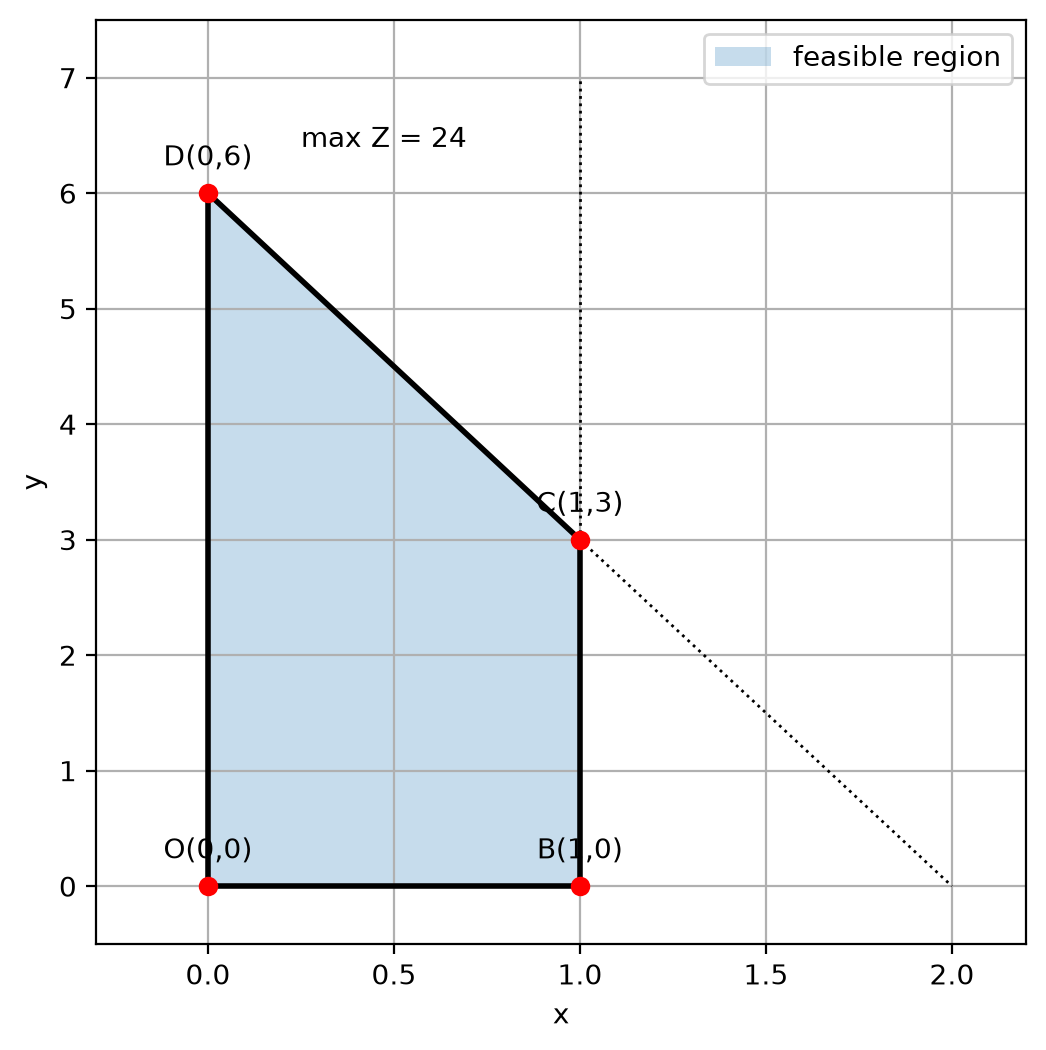
\includegraphics[width=0.5\linewidth]{figs/c12_q24.png}
	\caption{Feasible region and corner points}
	\label{fig:CBSE12-q24}
\end{figure}

\item
A box contains $10$ blocks: two marked $0$, three marked $1$, four marked $2$ and one marked $3$. A block is drawn at random. Find the probability distribution of the number $X$ on the block and its mean.
\hfill (CBSE Class 12, 65/7/1, Q.25(A))

\solution
Each block is equally likely, so the pmf is $\pr{X=x} = \frac{\text{number of blocks marked } x}{10}$:
\begin{table}[H]
	\centering
	\begin{tabular}{|c|c|c|c|c|}
		\hline
		$x$ & $0$ & $1$ & $2$ & $3$ \\ \hline
		$\pr{X=x}$ & $\frac{2}{10}$ & $\frac{3}{10}$ & $\frac{4}{10}$ & $\frac{1}{10}$ \\ \hline
	\end{tabular}
	\caption{Probability mass function of $X$}
	\label{tab:CBSE12-q25}
\end{table}
The probabilities sum to $1$. The mean is
\begin{align}
	E\sbrak{X} = \sum_x x\,\pr{X=x} = 0\brak{\frac{2}{10}} + 1\brak{\frac{3}{10}} + 2\brak{\frac{4}{10}} + 3\brak{\frac{1}{10}} = \frac{14}{10} = 1.4
\end{align}
The following code verifies the solution
\begin{lstlisting}[frame=single, basicstyle=\rmfamily, escapeinside={(*@}{@*)}]
(*@\makebox[\dimexpr\linewidth-2\fboxsep-2\fboxrule\relax][c]{codes/25.c}@*)
\end{lstlisting}

\item
Two ants move along the lines $2x + 5y - 1 = 0$ and $3x + 2y - 7 = 0$. Using the matrix method, find the point where their paths meet.
\hfill (CBSE Class 12, 65/7/1, Q.27(A))

\solution
In matrix form,
\begin{align}
	\myvec{2 & 5 \\ 3 & 2}\myvec{x \\ y} = \myvec{1 \\ 7}
\end{align}
The determinant is $2\brak{2} - 5\brak{3} = -11 \neq 0$, so the solution is unique. By Cramer's rule,
\begin{align}
	x = \frac{1\brak{2} - 5\brak{7}}{-11} = 3, \qquad y = \frac{2\brak{7} - 1\brak{3}}{-11} = -1
\end{align}
The paths meet at $\brak{3,-1}$.
The following code verifies the solution
\begin{lstlisting}[frame=single, basicstyle=\rmfamily, escapeinside={(*@}{@*)}]
(*@\makebox[\dimexpr\linewidth-2\fboxsep-2\fboxrule\relax][c]{codes/27.c}@*)
\end{lstlisting}

\item
Find $\dfrac{dy}{dx}$ if $y = \sqrt{\log\brak{\sin\brak{\frac{x^3}{3} - 1}}}$.
\hfill (CBSE Class 12, 65/7/1, Q.28)
% TODO: with log = ln, log(sin u) <= 0, so y is real only where sin u = 1;
% please check the exact expression in the paper.

\solution
Let $u = \frac{x^3}{3} - 1$, so $\frac{du}{dx} = x^2$. By the chain rule,
\begin{align}
	\frac{dy}{dx} &= \frac{1}{2\sqrt{\log\brak{\sin u}}}\cdot\frac{d}{dx}\log\brak{\sin u}
	= \frac{1}{2\sqrt{\log\brak{\sin u}}}\cdot\frac{\cos u}{\sin u}\cdot x^2
	\\
	&= \frac{x^2\cot\brak{\frac{x^3}{3}-1}}{2\sqrt{\log\brak{\sin\brak{\frac{x^3}{3}-1}}}}
\end{align}
The following code verifies the solution
\begin{lstlisting}[frame=single, basicstyle=\rmfamily, escapeinside={(*@}{@*)}]
(*@\makebox[\dimexpr\linewidth-2\fboxsep-2\fboxrule\relax][c]{codes/28.py}@*)
\end{lstlisting}

\item
Minimise $Z = 18x + 10y$ subject to $4x + y \ge 20$, $2x + 3y \ge 30$, $x \ge 0$, $y \ge 0$.
\hfill (CBSE Class 12, 65/7/1, Q.30)

\solution
The lines $4x + y = 20$ and $2x + 3y = 30$ meet where $y = 20 - 4x$ and $2x + 3\brak{20-4x} = 30$, so $x = 3$, $y = 8$. The feasible region is unbounded, with corner points $\brak{0,20}$, $\brak{3,8}$ and $\brak{15,0}$:
\begin{align}
	Z\brak{0,20} = 200, \qquad Z\brak{3,8} = 54 + 80 = 134, \qquad Z\brak{15,0} = 270
\end{align}
The minimum value is
\begin{align}
	Z_{\min} = 134 \text{ at } \brak{3,8}
\end{align}
The following code verifies the solution
\begin{lstlisting}[frame=single, basicstyle=\rmfamily, escapeinside={(*@}{@*)}]
(*@\makebox[\dimexpr\linewidth-2\fboxsep-2\fboxrule\relax][c]{codes/30.c}@*)
\end{lstlisting}
The following code generates \figref{fig:CBSE12-q30}.
\begin{lstlisting}[frame=single, basicstyle=\rmfamily, escapeinside={(*@}{@*)}]
(*@\makebox[\dimexpr\linewidth-2\fboxsep-2\fboxrule\relax][c]{codes/30plot.py}@*)
\end{lstlisting}
\begin{figure}[H]
	\centering
	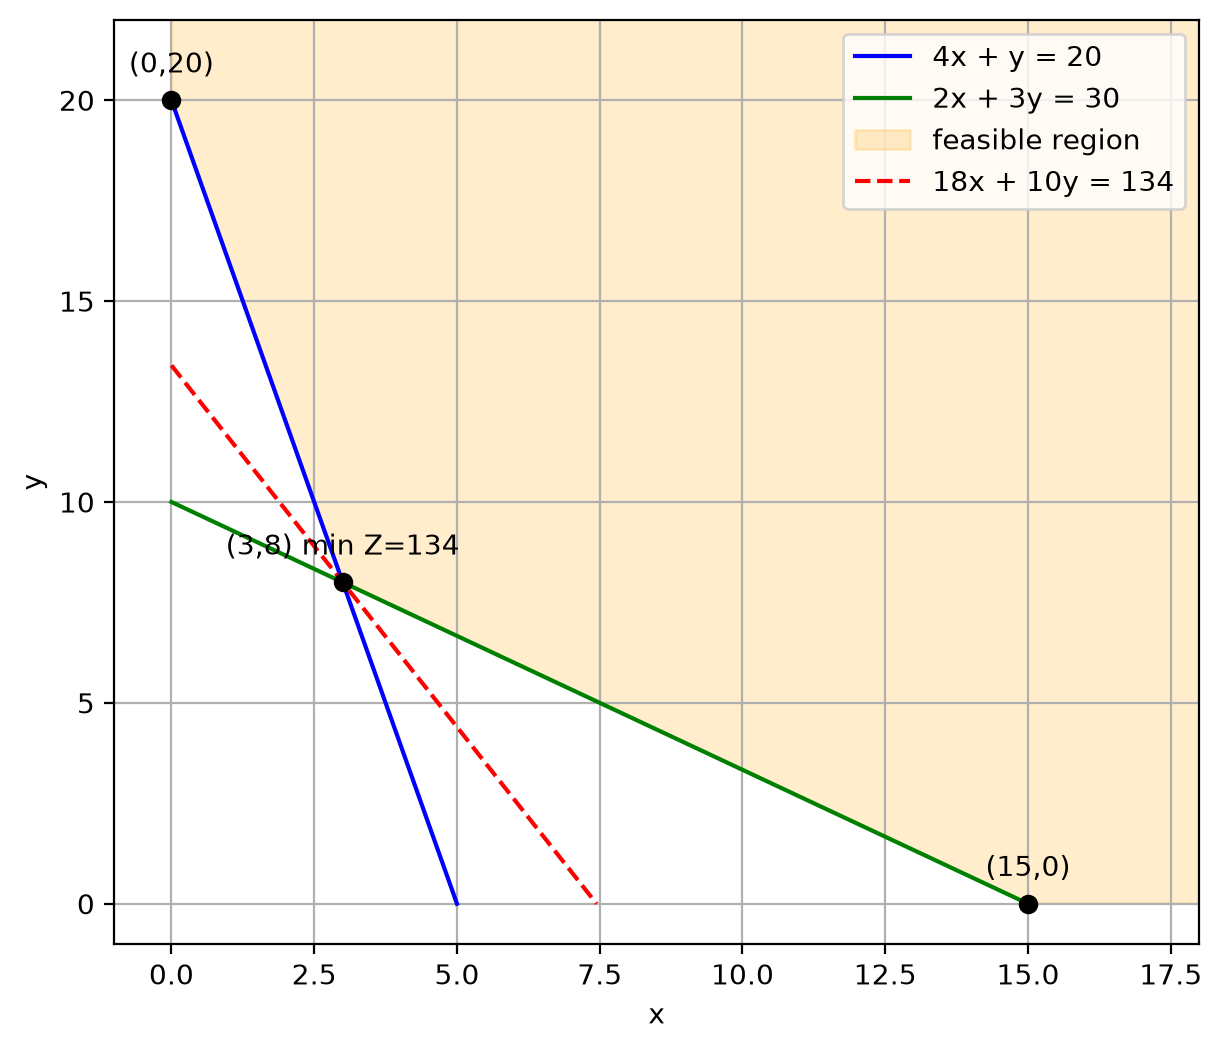
\includegraphics[width=0.6\linewidth]{figs/c12_q30.png}
	\caption{Unbounded feasible region and the line $Z = 134$}
	\label{fig:CBSE12-q30}
\end{figure}

\item
Let $\vec{a} = \hat{i} - \hat{j} + 2\hat{k}$, $\vec{b} = 2\hat{i} - 4\hat{j} + 5\hat{k}$ and $\vec{c} = \lambda\hat{i} - 2\hat{j} - 3\hat{k}$. Find $\lambda$ if the scalar product of $\vec{a}$ with the unit vector along $\vec{b} + \vec{c}$ is $1$.
\hfill (CBSE Class 12, 65/7/1, Q.31(A))

\solution
\begin{align}
	\vec{b} + \vec{c} = \myvec{\lambda+2 \\ -6 \\ 2}, \qquad \abs{\vec{b}+\vec{c}} = \sqrt{\brak{\lambda+2}^2 + 40}
\end{align}
The scalar product with $\vec{a} = \myvec{1\\-1\\2}$ is
\begin{align}
	\frac{\vec{a}^{\top}\brak{\vec{b}+\vec{c}}}{\abs{\vec{b}+\vec{c}}} = \frac{\lambda + 2 + 6 + 4}{\sqrt{\brak{\lambda+2}^2 + 40}} = \frac{\lambda+12}{\sqrt{\brak{\lambda+2}^2+40}} = 1
\end{align}
Squaring,
\begin{align}
	\brak{\lambda+12}^2 = \brak{\lambda+2}^2 + 40 \implies 20\lambda = -100 \implies \lambda = -5
\end{align}
Check: $\lambda + 12 = 7 > 0$ and $\sqrt{9 + 40} = 7$, so the unsquared equation holds.
The following code verifies the solution
\begin{lstlisting}[frame=single, basicstyle=\rmfamily, escapeinside={(*@}{@*)}]
(*@\makebox[\dimexpr\linewidth-2\fboxsep-2\fboxrule\relax][c]{codes/31A.c}@*)
\end{lstlisting}

\item
Find the shortest distance between the lines $\vec{r} = \brak{2\hat{i} - \hat{j} + 3\hat{k}} + \lambda\brak{\hat{i} - 2\hat{j} + 3\hat{k}}$ and $\vec{r} = \brak{\hat{i} + 4\hat{k}} + \mu\brak{3\hat{i} - 6\hat{j} + 9\hat{k}}$.
\hfill (CBSE Class 12, 65/7/1, Q.31(B))

\solution
The direction vectors $\vec{d}_1 = \myvec{1\\-2\\3}$ and $\vec{d}_2 = \myvec{3\\-6\\9} = 3\vec{d}_1$ are proportional, so the lines are parallel. Take $\vec{P}_1 = \myvec{2\\-1\\3}$ and $\vec{P}_2 = \myvec{1\\0\\4}$, so $\vec{P}_2 - \vec{P}_1 = \myvec{-1\\1\\1}$. The distance between parallel lines is
\begin{align}
	d = \frac{\norm{\brak{\vec{P}_2-\vec{P}_1}\times\vec{d}_1}}{\norm{\vec{d}_1}}
\end{align}
\begin{align}
	\myvec{-1\\1\\1}\times\myvec{1\\-2\\3} = \myvec{5\\4\\1}, \quad
	d = \frac{\sqrt{25+16+1}}{\sqrt{1+4+9}} = \frac{\sqrt{42}}{\sqrt{14}} = \sqrt{3}
\end{align}
The following code verifies the solution
\begin{lstlisting}[frame=single, basicstyle=\rmfamily, escapeinside={(*@}{@*)}]
(*@\makebox[\dimexpr\linewidth-2\fboxsep-2\fboxrule\relax][c]{codes/31B.c}@*)
\end{lstlisting}

\item
Evaluate $\displaystyle\int \frac{x^2 + 1}{\brak{x^2+2}\brak{2x^2+1}}\,dx$.
\hfill (CBSE Class 12, 65/7/1, Q.32(A))

\solution
Partial fractions in $x^2$:
\begin{align}
	\frac{x^2+1}{\brak{x^2+2}\brak{2x^2+1}} = \frac{A}{x^2+2} + \frac{B}{2x^2+1}
	\implies x^2 + 1 = A\brak{2x^2+1} + B\brak{x^2+2}
\end{align}
Comparing coefficients, $2A + B = 1$ and $A + 2B = 1$, so $A = B = \frac{1}{3}$. Using $\int\frac{dx}{x^2+a^2} = \frac{1}{a}\tan^{-1}\frac{x}{a}$,
\begin{align}
	\int \frac{x^2+1}{\brak{x^2+2}\brak{2x^2+1}}\,dx
	= \frac{1}{3\sqrt{2}}\tan^{-1}\brak{\frac{x}{\sqrt{2}}} + \frac{1}{3\sqrt{2}}\tan^{-1}\brak{\sqrt{2}\,x} + C
\end{align}
The program compares a midpoint Riemann sum over $\sbrak{0,1}$ with $F\brak{1}-F\brak{0} \approx 0.37024$. The following code verifies the solution
\begin{lstlisting}[frame=single, basicstyle=\rmfamily, escapeinside={(*@}{@*)}]
(*@\makebox[\dimexpr\linewidth-2\fboxsep-2\fboxrule\relax][c]{codes/32A.py}@*)
\end{lstlisting}
The following code generates \figref{fig:CBSE12-q32A}.
\begin{lstlisting}[frame=single, basicstyle=\rmfamily, escapeinside={(*@}{@*)}]
(*@\makebox[\dimexpr\linewidth-2\fboxsep-2\fboxrule\relax][c]{codes/32Aplot.py}@*)
\end{lstlisting}
\begin{figure}[H]
	\centering
	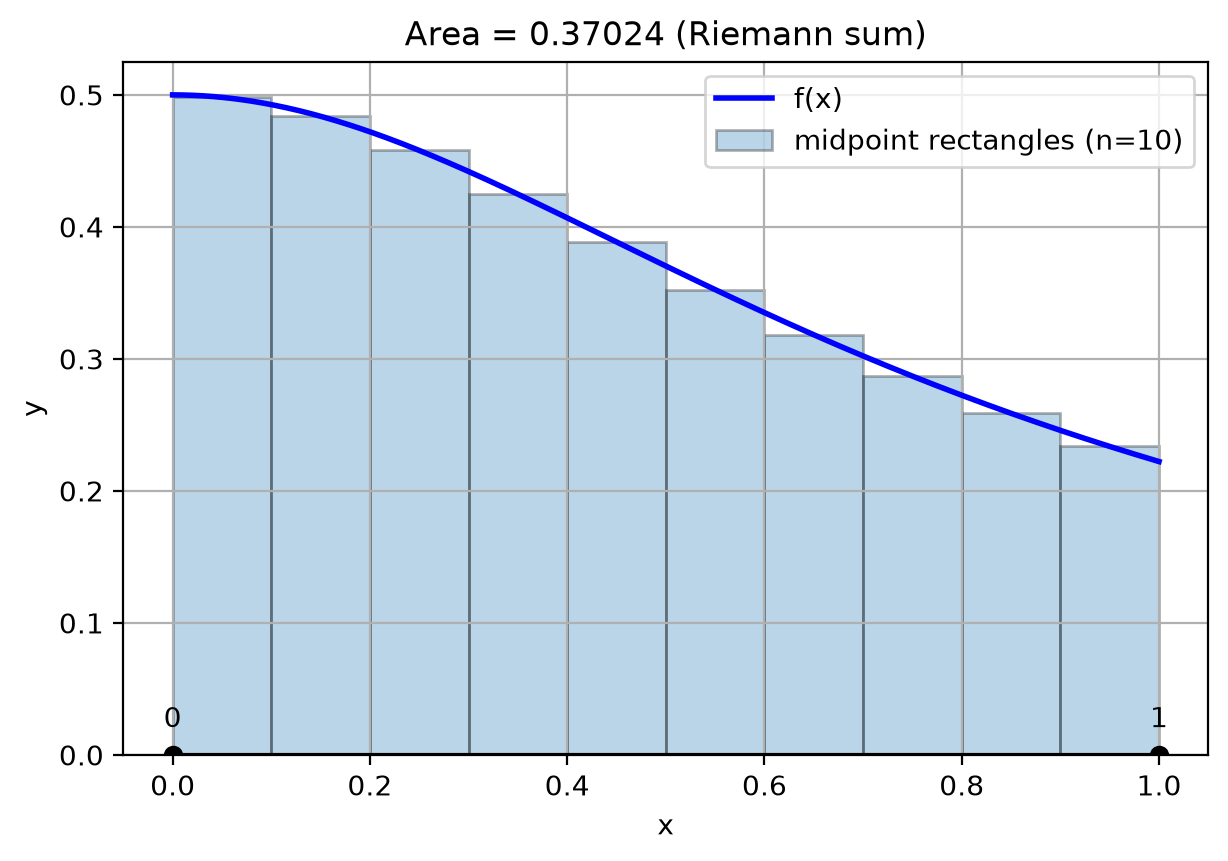
\includegraphics[width=0.6\linewidth]{figs/c12_q32A.png}
	\caption{Midpoint Riemann sum for $f\brak{x}$ on $\sbrak{0,1}$}
	\label{fig:CBSE12-q32A}
\end{figure}

\item
Evaluate $\displaystyle\int_0^{\pi} \frac{x\tan x}{\sec x + \tan x}\,dx$.
\hfill (CBSE Class 12, 65/7/1, Q.32(B))

\solution
Since $\frac{\tan x}{\sec x + \tan x} = \frac{\sin x}{1 + \sin x}$, the integral is $I = \int_0^\pi \frac{x\sin x}{1+\sin x}\,dx$. Using $\int_0^\pi xg\brak{x}\,dx = \frac{\pi}{2}\int_0^\pi g\brak{x}\,dx$ when $g\brak{\pi-x} = g\brak{x}$,
\begin{align}
	I = \frac{\pi}{2}\int_0^\pi \frac{\sin x}{1+\sin x}\,dx = \frac{\pi}{2}\int_0^\pi\brak{1 - \frac{1}{1+\sin x}}dx
\end{align}
Rationalising, $\frac{1}{1+\sin x} = \sec^2 x - \sec x\tan x$, whose antiderivative is $\tan x - \sec x$. Over $\sbrak{0,\pi}$ this gives $\int_0^\pi\frac{dx}{1+\sin x} = 2$ (the point $x = \frac{\pi}{2}$ is handled by taking limits on either side). Hence
\begin{align}
	I = \frac{\pi}{2}\brak{\pi - 2} \approx 1.7932
\end{align}
The following code verifies the solution
\begin{lstlisting}[frame=single, basicstyle=\rmfamily, escapeinside={(*@}{@*)}]
(*@\makebox[\dimexpr\linewidth-2\fboxsep-2\fboxrule\relax][c]{codes/32B.py}@*)
\end{lstlisting}
The following code generates \figref{fig:CBSE12-q32B}.
\begin{lstlisting}[frame=single, basicstyle=\rmfamily, escapeinside={(*@}{@*)}]
(*@\makebox[\dimexpr\linewidth-2\fboxsep-2\fboxrule\relax][c]{codes/32Bplot.py}@*)
\end{lstlisting}
\begin{figure}[H]
	\centering
	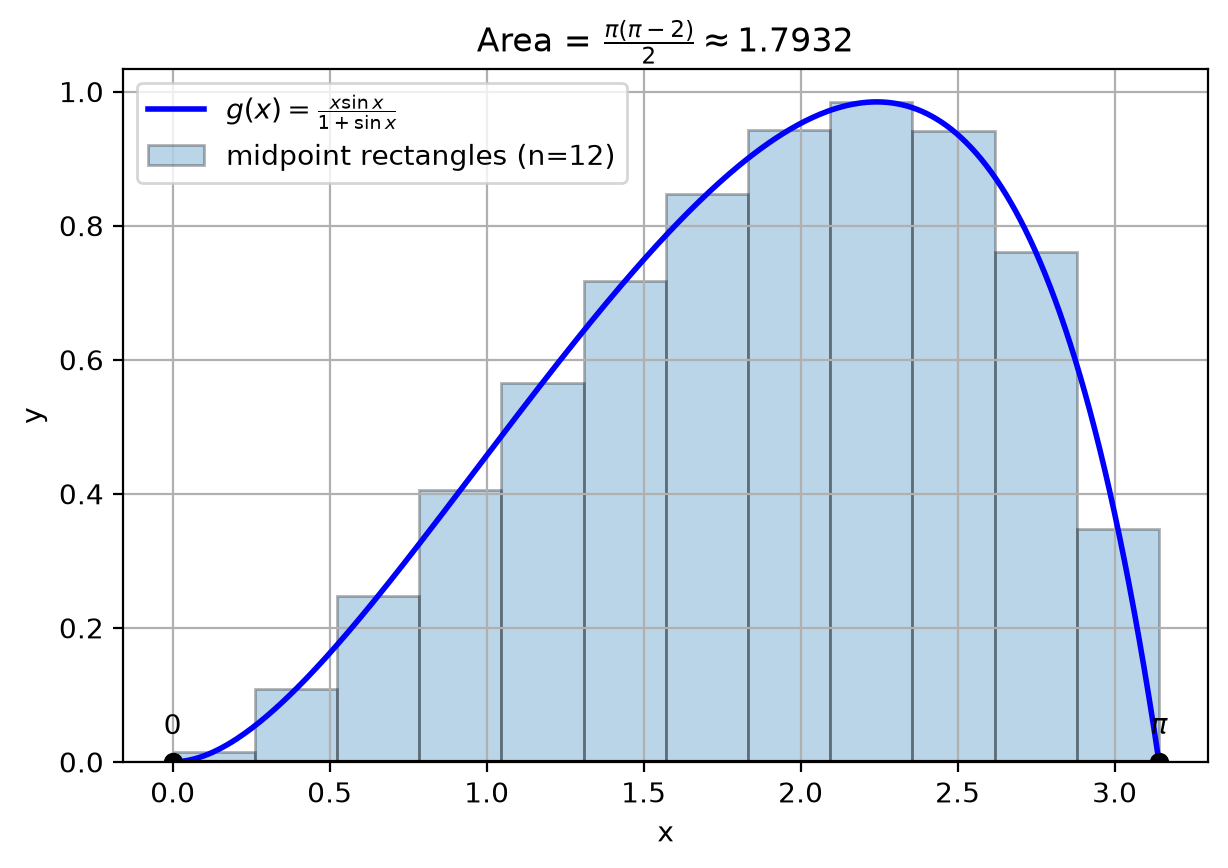
\includegraphics[width=0.6\linewidth]{figs/c12_q32B.png}
	\caption{Midpoint Riemann sum for $\frac{x\sin x}{1+\sin x}$ on $\sbrak{0,\pi}$}
	\label{fig:CBSE12-q32B}
\end{figure}

\item
Solve $\dfrac{dy}{dx} = \cos x - 2y$ using Laplace transforms.
\hfill (CBSE Class 12, 65/7/1, Q.34)

\solution
Rewrite as $y^{\prime} + 2y = \cos x$ and let $Y\brak{s} = \mathcal{L}\cbrak{y}$, $y\brak{0} = y_0$. Since $\mathcal{L}\cbrak{y^{\prime}} = sY - y_0$ and $\mathcal{L}\cbrak{\cos x} = \frac{s}{s^2+1}$,
\begin{align}
	\brak{s+2}Y\brak{s} = y_0 + \frac{s}{s^2+1} \implies Y\brak{s} = \frac{y_0}{s+2} + \frac{s}{\brak{s+2}\brak{s^2+1}}
\end{align}
Partial fractions: $\frac{s}{\brak{s+2}\brak{s^2+1}} = \frac{-\frac{2}{5}}{s+2} + \frac{\frac{2}{5}s + \frac{1}{5}}{s^2+1}$. Using $\mathcal{L}^{-1}\cbrak{\frac{1}{s+2}} = e^{-2x}$, $\mathcal{L}^{-1}\cbrak{\frac{s}{s^2+1}} = \cos x$ and $\mathcal{L}^{-1}\cbrak{\frac{1}{s^2+1}} = \sin x$,
\begin{align}
	y\brak{x} = \brak{y_0 - \frac{2}{5}}e^{-2x} + \frac{2}{5}\cos x + \frac{1}{5}\sin x = Ce^{-2x} + \frac{2\cos x + \sin x}{5}
\end{align}
No initial condition is given, so the constant $C$ is arbitrary. The following code verifies the solution
\begin{lstlisting}[frame=single, basicstyle=\rmfamily, escapeinside={(*@}{@*)}]
(*@\makebox[\dimexpr\linewidth-2\fboxsep-2\fboxrule\relax][c]{codes/34.py}@*)
\end{lstlisting}

\item
Find the points on the line $\dfrac{2x+4}{6} = \dfrac{y+1}{2} = \dfrac{-2z+6}{-4}$ at a distance of $3\sqrt{2}$ units from the point $P\brak{1,2,3}$.
\hfill (CBSE Class 12, 65/7/1, Q.35(A))

\solution
Let the common ratio be $t$. Then $x = 3t - 2$, $y = 2t - 1$, $z = 2t + 3$. The squared distance from $P$ is
\begin{align}
	\brak{3t-3}^2 + \brak{2t-3}^2 + \brak{2t}^2 = 17t^2 - 30t + 18 = 18
\end{align}
\begin{align}
	t\brak{17t - 30} = 0 \implies t = 0 \text{ or } t = \frac{30}{17}
\end{align}
The required points are
\begin{align}
	Q_1 = \brak{-2,-1,3}, \qquad Q_2 = \brak{\frac{56}{17}, \frac{43}{17}, \frac{111}{17}}
\end{align}
The following code verifies the solution
\begin{lstlisting}[frame=single, basicstyle=\rmfamily, escapeinside={(*@}{@*)}]
(*@\makebox[\dimexpr\linewidth-2\fboxsep-2\fboxrule\relax][c]{codes/35A.c}@*)
\end{lstlisting}
The following code generates \figref{fig:CBSE12-q35A}.
\begin{lstlisting}[frame=single, basicstyle=\rmfamily, escapeinside={(*@}{@*)}]
(*@\makebox[\dimexpr\linewidth-2\fboxsep-2\fboxrule\relax][c]{codes/35Aplot.py}@*)
\end{lstlisting}
\begin{figure}[H]
	\centering
	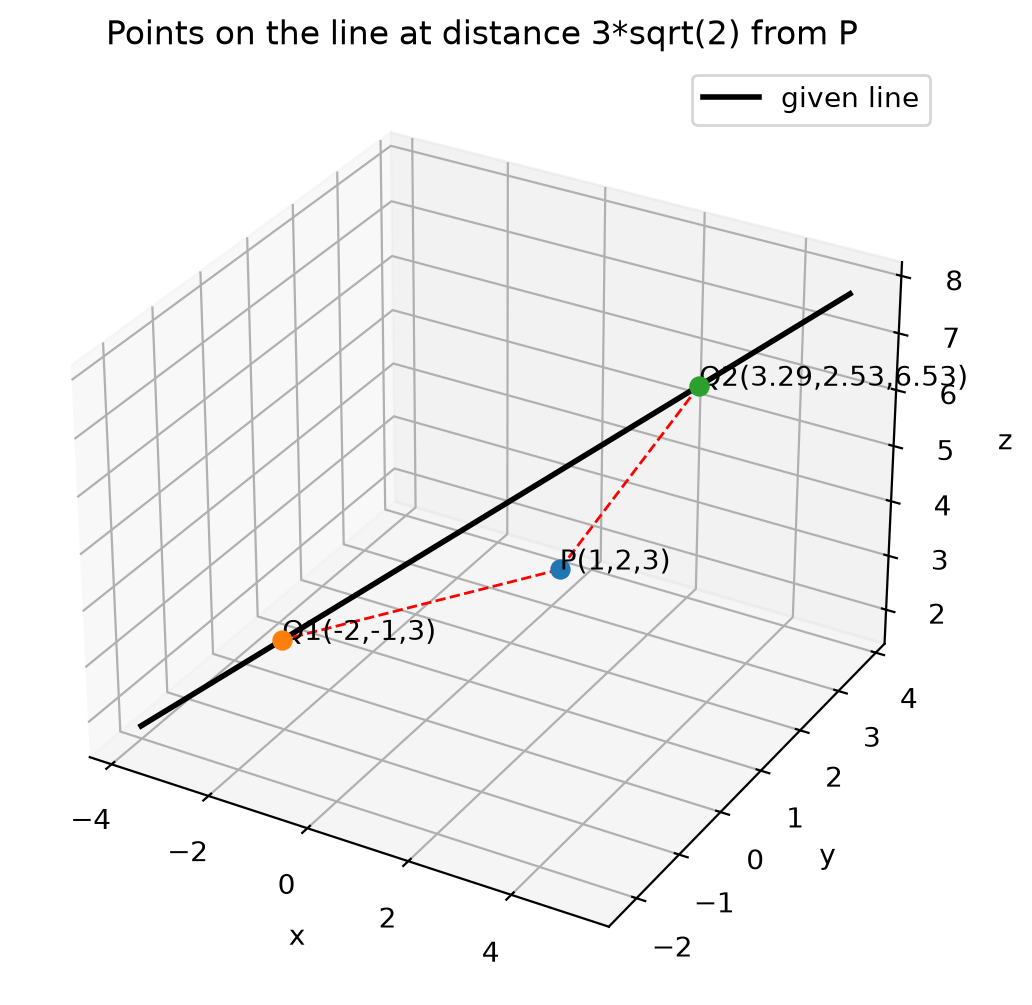
\includegraphics[width=0.6\linewidth]{figs/c12_q35A.png}
	\caption{Points $Q_1$, $Q_2$ on the line at distance $3\sqrt{2}$ from $P$}
	\label{fig:CBSE12-q35A}
\end{figure}

\item
Find the image of the point $P\brak{-1,5,2}$ in the line $\dfrac{2x-4}{2} = \dfrac{y}{2} = \dfrac{2-z}{3}$, and the length $PP^{\prime}$.
\hfill (CBSE Class 12, 65/7/1, Q.35(B))

\solution
Let the common ratio be $t$: $x = t + 2$, $y = 2t$, $z = 2 - 3t$. The line passes through $\vec{A} = \myvec{2\\0\\2}$ with direction $\vec{d} = \myvec{1\\2\\-3}$. The foot of the perpendicular $H = \vec{A} + t_0\vec{d}$ has
\begin{align}
	t_0 = \frac{\brak{\vec{P}-\vec{A}}^{\top}\vec{d}}{\vec{d}^{\top}\vec{d}} = \frac{\myvec{-3\\5\\0}^{\top}\myvec{1\\2\\-3}}{14} = \frac{7}{14} = \frac{1}{2}
	\implies \vec{H} = \myvec{\frac{5}{2}\\1\\\frac{1}{2}}
\end{align}
Since $H$ is the mid-point of $PP^{\prime}$,
\begin{align}
	\vec{P}^{\prime} = 2\vec{H} - \vec{P} = \myvec{5\\2\\1} - \myvec{-1\\5\\2} = \myvec{6\\-3\\-1}
\end{align}
\begin{align}
	PP^{\prime} = \sqrt{7^2 + 8^2 + 3^2} = \sqrt{122}
\end{align}
The following code verifies the solution
\begin{lstlisting}[frame=single, basicstyle=\rmfamily, escapeinside={(*@}{@*)}]
(*@\makebox[\dimexpr\linewidth-2\fboxsep-2\fboxrule\relax][c]{codes/35B.c}@*)
\end{lstlisting}
The following code generates \figref{fig:CBSE12-q35B}.
\begin{lstlisting}[frame=single, basicstyle=\rmfamily, escapeinside={(*@}{@*)}]
(*@\makebox[\dimexpr\linewidth-2\fboxsep-2\fboxrule\relax][c]{codes/35Bplot.py}@*)
\end{lstlisting}
\begin{figure}[H]
	\centering
	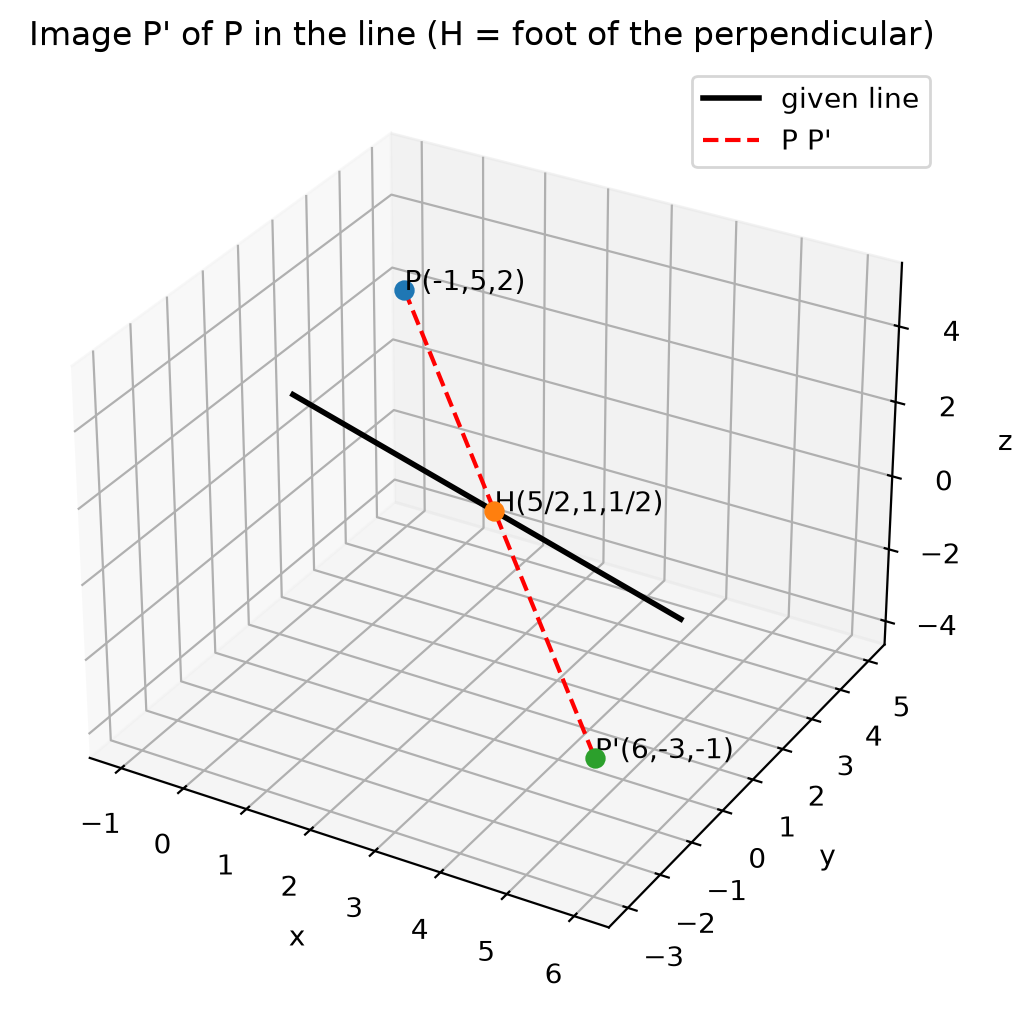
\includegraphics[width=0.6\linewidth]{figs/c12_q35B.png}
	\caption{Point $P$, its image $P^{\prime}$ and the foot $H$}
	\label{fig:CBSE12-q35B}
\end{figure}

\item
\textbf{Case study (camphor).} The radius $r$ of a camphor tablet decreases with time $t$ (in hours) as it evaporates, and $\frac{dr}{dt} = -\frac{2}{3}k$ with $k > 0$ and $r\brak{0} = 5$ mm. (i) Write the order and degree of the differential equation. (ii) Solve it using the Laplace transform. (iii)(a) If $r = 3$ mm after $1$ hour, find the time for the radius to become $0$. \textbf{OR} (iii)(b) If $r = 1$ mm after $1$ hour, find the time for the radius to become $0$.
\hfill (CBSE Class 12, 65/7/1, Q.37)
% NOTE: the chat printed t = 2 hours for part (iii)(a); the correct value is 5/2 hours.
% TODO: the paper prints dr/dt = +(2/3)k; the sign is taken negative so that r decreases.

\solution
\textbf{(i)} The highest derivative is $\frac{dr}{dt}$ and its power is $1$, so the order is $1$ and the degree is $1$.

\textbf{(ii)} Let $R\brak{s} = \mathcal{L}\cbrak{r}$. Then
\begin{align}
	sR\brak{s} - r\brak{0} = -\frac{2k}{3s} \implies R\brak{s} = \frac{5}{s} - \frac{2k}{3s^2}
	\implies r\brak{t} = 5 - \frac{2}{3}kt
\end{align}
\textbf{(iii)(a)} From $r\brak{1} = 3$: $3 = 5 - \frac{2}{3}k \implies k = 3$, so $r\brak{t} = 5 - 2t$. Setting $r = 0$,
\begin{align}
	t = \frac{5}{2} \text{ hours}
\end{align}
\textbf{(iii)(b)} From $r\brak{1} = 1$: $1 = 5 - \frac{2}{3}k \implies k = 6$, so $r\brak{t} = 5 - 4t$ and
\begin{align}
	t = \frac{5}{4} \text{ hours}
\end{align}
The following code verifies the solution
\begin{lstlisting}[frame=single, basicstyle=\rmfamily, escapeinside={(*@}{@*)}]
(*@\makebox[\dimexpr\linewidth-2\fboxsep-2\fboxrule\relax][c]{codes/37.c}@*)
\end{lstlisting}

\item
\textbf{Case study (health survey).} Of $1000$ people, $700$ have good health ($A_1$), $200$ average health ($A_2$) and $100$ poor health ($A_3$). The probabilities of contracting the disease $D$ are $\pr{D\mid A_1} = 0.25$, $\pr{D\mid A_2} = 0.35$ and $\pr{D\mid A_3} = 0.50$. (i) Find the probability that a randomly selected person has contracted the disease. (ii) Find the probability that a person who has not contracted the disease belongs to category $A_1$.
\hfill (CBSE Class 12, 65/7/1, Q.38)

\solution
The mapping from category to probability is $\pr{A_1} = 0.7$, $\pr{A_2} = 0.2$, $\pr{A_3} = 0.1$, and these sum to $1$.

\textbf{(i)} By the law of total probability,
\begin{align}
	\pr{D} = \sum_{i=1}^{3}\pr{D\mid A_i}\pr{A_i} = 0.25\brak{0.7} + 0.35\brak{0.2} + 0.50\brak{0.1} = 0.295
\end{align}
\textbf{(ii)} $\pr{D^{\prime}} = 1 - 0.295 = 0.705$ and $\pr{D^{\prime}\mid A_1} = 0.75$. By Bayes' theorem,
\begin{align}
	\pr{A_1\mid D^{\prime}} = \frac{\pr{D^{\prime}\mid A_1}\pr{A_1}}{\pr{D^{\prime}}} = \frac{0.75\brak{0.7}}{0.705} = \frac{0.525}{0.705} = \frac{35}{47} \approx 0.7447
\end{align}
The following code verifies the solution
\begin{lstlisting}[frame=single, basicstyle=\rmfamily, escapeinside={(*@}{@*)}]
(*@\makebox[\dimexpr\linewidth-2\fboxsep-2\fboxrule\relax][c]{codes/38.c}@*)
\end{lstlisting}

\end{enumerate}
